\chapter{The Colosseum}

Franz had so managed his route, that during the ride to the Colosseum
they passed not a single ancient ruin, so that no preliminary
impression interfered to mitigate the colossal proportions of the
gigantic building they came to admire. The road selected was a
continuation of the Via Sistina; then by cutting off the right angle of
the street in which stands Santa Maria Maggiore and proceeding by the
Via Urbana and San Pietro in Vincoli, the travellers would find
themselves directly opposite the Colosseum.

This itinerary possessed another great advantage,—that of leaving Franz
at full liberty to indulge his deep reverie upon the subject of Signor
Pastrini’s story, in which his mysterious host of Monte Cristo was so
strangely mixed up. Seated with folded arms in a corner of the
carriage, he continued to ponder over the singular history he had so
lately listened to, and to ask himself an interminable number of
questions touching its various circumstances without, however, arriving
at a satisfactory reply to any of them.

One fact more than the rest brought his friend “Sinbad the Sailor” back
to his recollection, and that was the mysterious sort of intimacy that
seemed to exist between the brigands and the sailors; and Pastrini’s
account of Vampa’s having found refuge on board the vessels of
smugglers and fishermen, reminded Franz of the two Corsican bandits he
had found supping so amicably with the crew of the little yacht, which
had even deviated from its course and touched at Porto-Vecchio for the
sole purpose of landing them. The very name assumed by his host of
Monte Cristo and again repeated by the landlord of the Hôtel de
Londres, abundantly proved to him that his island friend was playing
his philanthropic part on the shores of Piombino, Civita Vecchia,
Ostia, and Gaëta, as on those of Corsica, Tuscany, and Spain; and
further, Franz bethought him of having heard his singular entertainer
speak both of Tunis and Palermo, proving thereby how largely his circle
of acquaintances extended.

But however the mind of the young man might be absorbed in these
reflections, they were at once dispersed at the sight of the dark
frowning ruins of the stupendous Colosseum, through the various
openings of which the pale moonlight played and flickered like the
unearthly gleam from the eyes of the wandering dead. The carriage
stopped near the Meta Sudans; the door was opened, and the young men,
eagerly alighting, found themselves opposite a \textit{cicerone}, who appeared
to have sprung up from the ground, so unexpected was his appearance.

The usual guide from the hotel having followed them, they had paid two
conductors, nor is it possible, at Rome, to avoid this abundant supply
of guides; besides the ordinary \textit{cicerone}, who seizes upon you
directly you set foot in your hotel, and never quits you while you
remain in the city, there is also a special \textit{cicerone} belonging to
each monument—nay, almost to each part of a monument. It may,
therefore, be easily imagined there is no scarcity of guides at the
Colosseum, that wonder of all ages, which Martial thus eulogizes:

“Let Memphis cease to boast the barbarous miracles of her pyramids, and
the wonders of Babylon be talked of no more among us; all must bow to
the superiority of the gigantic labor of the Cæsars, and the many
voices of Fame spread far and wide the surpassing merits of this
incomparable monument.”

As for Albert and Franz, they essayed not to escape from their
\textit{ciceronian} tyrants; and, indeed, it would have been so much the more
difficult to break their bondage, as the guides alone are permitted to
visit these monuments with torches in their hands. Thus, then, the
young men made no attempt at resistance, but blindly and confidingly
surrendered themselves into the care and custody of their conductors.

Franz had already made seven or eight similar excursions to the
Colosseum, while his less favored companion trod for the first time in
his life the classic ground forming the monument of Flavius Vespasian;
and, to his credit be it spoken, his mind, even amid the glib loquacity
of the guides, was duly and deeply touched with awe and enthusiastic
admiration of all he saw; and certainly no adequate notion of these
stupendous ruins can be formed save by such as have visited them, and
more especially by moonlight, at which time the vast proportions of the
building appear twice as large when viewed by the mysterious beams of a
southern moonlit sky, whose rays are sufficiently clear and vivid to
light the horizon with a glow equal to the soft twilight of a western
clime.

Scarcely, therefore, had the reflective Franz walked a hundred steps
beneath the interior porticoes of the ruin, when, abandoning Albert to
the guides (who would by no means yield their prescriptive right of
carrying their victims through the routine regularly laid down, and as
regularly followed by them, but dragged the unconscious visitor to the
various objects with a pertinacity that admitted of no appeal,
beginning, as a matter of course, with the “Lions’ Den”, the “Hall of
the Gladiators” and finishing with “Cæsar’s Podium”), to escape a
jargon and mechanical survey of the wonders by which he was surrounded,
Franz ascended a half-dilapidated staircase, and, leaving them to
follow their monotonous round, seated himself at the foot of a column,
and immediately opposite a large aperture, which permitted him to enjoy
a full and undisturbed view of the gigantic dimensions of the majestic
ruin.

Franz had remained for nearly a quarter of an hour perfectly hidden by
the shadow of the vast column at whose base he had found a
resting-place, and from whence his eyes followed the motions of Albert
and his guides, who, holding torches in their hands, had emerged from a
vomitorium at the opposite extremity of the Colosseum, and then again
disappeared down the steps conducting to the seats reserved for the
Vestal virgins, resembling, as they glided along, some restless shades
following the flickering glare of so many \textit{ignes fatui}. All at once
his ear caught a sound resembling that of a stone rolling down the
staircase opposite the one by which he had himself ascended. There was
nothing remarkable in the circumstance of a fragment of granite giving
way and falling heavily below; but it seemed to him that the substance
that fell gave way beneath the pressure of a foot, and also that
someone, who endeavored as much as possible to prevent his footsteps
from being heard, was approaching the spot where he sat.

Conjecture soon became certainty, for the figure of a man was
distinctly visible to Franz, gradually emerging from the staircase
opposite, upon which the moon was at that moment pouring a full tide of
silvery brightness.

The stranger thus presenting himself was probably a person who, like
Franz, preferred the enjoyment of solitude and his own thoughts to the
frivolous gabble of the guides. And his appearance had nothing
extraordinary in it; but the hesitation with which he proceeded,
stopping and listening with anxious attention at every step he took,
convinced Franz that he expected the arrival of some person.

By a sort of instinctive impulse, Franz withdrew as much as possible
behind his pillar.

About ten feet from the spot where he and the stranger were, the roof
had given way, leaving a large round opening, through which might be
seen the blue vault of heaven, thickly studded with stars.

Around this opening, which had, possibly, for ages permitted a free
entrance to the brilliant moonbeams that now illumined the vast pile,
grew a quantity of creeping plants, whose delicate green branches stood
out in bold relief against the clear azure of the firmament, while
large masses of thick, strong fibrous shoots forced their way through
the chasm, and hung floating to and fro, like so many waving strings.

The person whose mysterious arrival had attracted the attention of
Franz stood in a kind of half-light, that rendered it impossible to
distinguish his features, although his dress was easily made out. He
wore a large brown mantle, one fold of which, thrown over his left
shoulder, served likewise to mask the lower part of his countenance,
while the upper part was completely hidden by his broad-brimmed hat.
The lower part of his dress was more distinctly visible by the bright
rays of the moon, which, entering through the broken ceiling, shed
their refulgent beams on feet cased in elegantly made boots of polished
leather, over which descended fashionably cut trousers of black cloth.

\begin{figure}[ht]
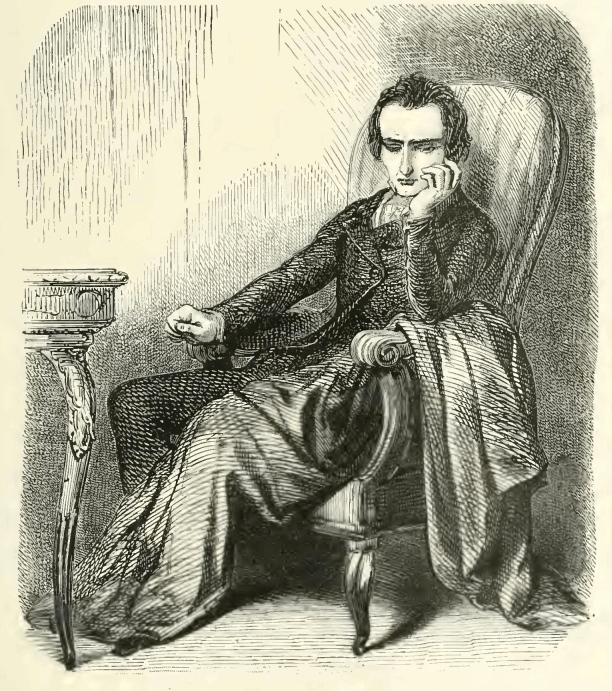
\includegraphics[width=\textwidth]{20135m.jpg}
\end{figure}

From the imperfect means Franz had of judging, he could only come to
one conclusion,—that the person whom he was thus watching certainly
belonged to no inferior station of life.

Some few minutes had elapsed, and the stranger began to show manifest
signs of impatience, when a slight noise was heard outside the aperture
in the roof, and almost immediately a dark shadow seemed to obstruct
the flood of light that had entered it, and the figure of a man was
clearly seen gazing with eager scrutiny on the immense space beneath
him; then, as his eye caught sight of him in the mantle, he grasped a
floating mass of thickly matted boughs, and glided down by their help
to within three or four feet of the ground, and then leaped lightly on
his feet. The man who had performed this daring act with so much
indifference wore the Transtevere costume.

“I beg your excellency’s pardon for keeping you waiting,” said the man,
in the Roman dialect, “but I don’t think I’m many minutes after my
time, ten o’clock has just struck by the clock of Saint John Lateran.”

“Say not a word about being late,” replied the stranger in purest
Tuscan; “’tis I who am too soon. But even if you had caused me to wait
a little while, I should have felt quite sure that the delay was not
occasioned by any fault of yours.”

“Your excellency is perfectly right in so thinking,” said the man; “I
came here direct from the Castle of St. Angelo, and I had an immense
deal of trouble before I could get a chance to speak to Beppo.”

“And who is Beppo?”

“Oh, Beppo is employed in the prison, and I give him so much a year to
let me know what is going on within his holiness’s castle.”

“Indeed! You are a provident person, I see.”

“Why, you see, no one knows what may happen. Perhaps some of these days
I may be entrapped, like poor Peppino and may be very glad to have some
little nibbling mouse to gnaw the meshes of my net, and so help me out
of prison.”

“Briefly, what did you learn?”

“That two executions of considerable interest will take place the day
after tomorrow at two o’clock, as is customary at Rome at the
commencement of all great festivals. One of the culprits will be
\textit{mazzolato};3 he is an atrocious villain, who murdered the priest who
brought him up, and deserves not the smallest pity. The other sufferer
is sentenced to be \textit{decapitato};4 and he, your excellency, is poor
Peppino.”

“The fact is, that you have inspired not only the pontifical
government, but also the neighboring states, with such extreme fear,
that they are glad of all opportunity of making an example.”

“But Peppino did not even belong to my band; he was merely a poor
shepherd, whose only crime consisted in furnishing us with provisions.”

“Which makes him your accomplice to all intents and purposes. But mark
the distinction with which he is treated; instead of being knocked on
the head as you would be if once they caught hold of you, he is simply
sentenced to be guillotined, by which means, too, the amusements of the
day are diversified, and there is a spectacle to please every
spectator.”

“Without reckoning the wholly unexpected one I am preparing to surprise
them with.”

“My good friend,” said the man in the cloak, “excuse me for saying that
you seem to me precisely in the mood to commit some wild or extravagant
act.”

“Perhaps I am; but one thing I have resolved on, and that is, to stop
at nothing to restore a poor devil to liberty, who has got into this
scrape solely from having served me. I should hate and despise myself
as a coward did I desert the brave fellow in his present extremity.”

“And what do you mean to do?”

“To surround the scaffold with twenty of my best men, who, at a signal
from me, will rush forward directly Peppino is brought for execution,
and, by the assistance of their stilettos, drive back the guard, and
carry off the prisoner.”

“That seems to me as hazardous as uncertain, and convinces me that my
scheme is far better than yours.”

“And what is your excellency’s project?”

“Just this. I will so advantageously bestow 2,000 piastres, that the
person receiving them shall obtain a respite till next year for
Peppino; and during that year, another skilfully placed 1,000 piastres
will afford him the means of escaping from his prison.”

“And do you feel sure of succeeding?”

“\textit{Pardieu!}” exclaimed the man in the cloak, suddenly expressing
himself in French.

“What did your excellency say?” inquired the other.

“I said, my good fellow, that I would do more single-handed by the
means of gold than you and all your troop could effect with stilettos,
pistols, carbines, and blunderbusses included. Leave me, then, to act,
and have no fears for the result.”

“At least, there can be no harm in myself and party being in readiness,
in case your excellency should fail.”

“None whatever. Take what precautions you please, if it is any
satisfaction to you to do so; but rely upon my obtaining the reprieve I
seek.”

“Remember, the execution is fixed for the day after tomorrow, and that
you have but one day to work in.”

“And what of that? Is not a day divided into twenty-four hours, each
hour into sixty minutes, and every minute sub-divided into sixty
seconds? Now in 86,400 seconds very many things can be done.”

“And how shall I know whether your excellency has succeeded or not.”

“Oh, that is very easily arranged. I have engaged the three lower
windows at the Café Rospoli; should I have obtained the requisite
pardon for Peppino, the two outside windows will be hung with yellow
damasks, and the centre with white, having a large cross in red marked
on it.”

“And whom will you employ to carry the reprieve to the officer
directing the execution?”

“Send one of your men, disguised as a penitent friar, and I will give
it to him. His dress will procure him the means of approaching the
scaffold itself, and he will deliver the official order to the officer,
who, in his turn, will hand it to the executioner; in the meantime, it
will be as well to acquaint Peppino with what we have determined on, if
it be only to prevent his dying of fear or losing his senses, because
in either case a very useless expense will have been incurred.”

“Your excellency,” said the man, “you are fully persuaded of my entire
devotion to you, are you not?”

“Nay, I flatter myself that there can be no doubt of it,” replied the
cavalier in the cloak.

“Well, then, only fulfil your promise of rescuing Peppino, and
henceforward you shall receive not only devotion, but the most absolute
obedience from myself and those under me that one human being can
render to another.”

“Have a care how far you pledge yourself, my good friend, for I may
remind you of your promise at some, perhaps, not very distant period,
when I, in my turn, may require your aid and influence.”

“Let that day come sooner or later, your excellency will find me what I
have found you in this my heavy trouble; and if from the other end of
the world you but write me word to do such or such a thing, you may
regard it as done, for done it shall be, on the word and faith of——”

“Hush!” interrupted the stranger; “I hear a noise.”

“’Tis some travellers, who are visiting the Colosseum by torchlight.”

“’Twere better we should not be seen together; those guides are nothing
but spies, and might possibly recognize you; and, however I may be
honored by your friendship, my worthy friend, if once the extent of our
intimacy were known, I am sadly afraid both my reputation and credit
would suffer thereby.”

“Well, then, if you obtain the reprieve?”

“The middle window at the Café Rospoli will be hung with white damask,
bearing a red cross.”

“And if you fail?”

“Then all three windows will have yellow draperies.”

“And then?”

“And then, my good fellow, use your daggers in any way you please, and
I further promise you to be there as a spectator of your prowess.”

“We understand each other perfectly, then. Adieu, your excellency;
depend upon me as firmly as I do upon you.”

Saying these words, the Transteverin disappeared down the staircase,
while his companion, muffling his features more closely than before in
the folds of his mantle, passed almost close to Franz, and descended to
the arena by an outward flight of steps. The next minute Franz heard
himself called by Albert, who made the lofty building re-echo with the
sound of his friend’s name. Franz, however, did not obey the summons
till he had satisfied himself that the two men whose conversation he
had overheard were at a sufficient distance to prevent his encountering
them in his descent. In ten minutes after the strangers had departed,
Franz was on the road to the Piazza di Spagna, listening with studied
indifference to the learned dissertation delivered by Albert, after the
manner of Pliny and Calpurnius, touching the iron-pointed nets used to
prevent the ferocious beasts from springing on the spectators.

Franz let him proceed without interruption, and, in fact, did not hear
what was said; he longed to be alone, and free to ponder over all that
had occurred. One of the two men, whose mysterious meeting in the
Colosseum he had so unintentionally witnessed, was an entire stranger
to him, but not so the other; and though Franz had been unable to
distinguish his features, from his being either wrapped in his mantle
or obscured by the shadow, the tones of his voice had made too powerful
an impression on him the first time he had heard them for him ever
again to forget them, hear them when or where he might. It was more
especially when this man was speaking in a manner half jesting, half
bitter, that Franz’s ear recalled most vividly the deep sonorous, yet
well-pitched voice that had addressed him in the grotto of Monte
Cristo, and which he heard for the second time amid the darkness and
ruined grandeur of the Colosseum. And the more he thought, the more
entire was his conviction, that the person who wore the mantle was no
other than his former host and entertainer, “Sinbad the Sailor.”

\begin{figure}[ht]
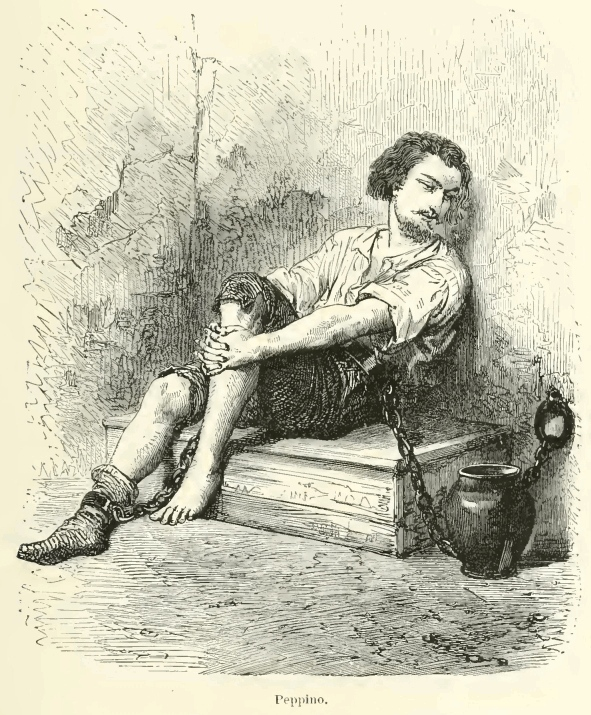
\includegraphics[width=\textwidth]{20139m.jpg}
\end{figure}

Under any other circumstances, Franz would have found it impossible to
resist his extreme curiosity to know more of so singular a personage,
and with that intent have sought to renew their short acquaintance; but
in the present instance, the confidential nature of the conversation he
had overheard made him, with propriety, judge that his appearance at
such a time would be anything but agreeable. As we have seen,
therefore, he permitted his former host to retire without attempting a
recognition, but fully promising himself a rich indemnity for his
present forbearance should chance afford him another opportunity.

In vain did Franz endeavor to forget the many perplexing thoughts which
assailed him; in vain did he court the refreshment of sleep. Slumber
refused to visit his eyelids and the night was passed in feverish
contemplation of the chain of circumstances tending to prove the
identity of the mysterious visitant to the Colosseum with the
inhabitant of the grotto of Monte Cristo; and the more he thought, the
firmer grew his opinion on the subject.

Worn out at length, he fell asleep at daybreak, and did not awake till
late. Like a genuine Frenchman, Albert had employed his time in
arranging for the evening’s diversion; he had sent to engage a box at
the Teatro Argentina; and Franz, having a number of letters to write,
relinquished the carriage to Albert for the whole of the day.

At five o’clock Albert returned, delighted with his day’s work; he had
been occupied in leaving his letters of introduction, and had received
in return more invitations to balls and routs than it would be possible
for him to accept; besides this, he had seen (as he called it) all the
remarkable sights at Rome. Yes, in a single day he had accomplished
what his more serious-minded companion would have taken weeks to
effect. Neither had he neglected to ascertain the name of the piece to
be played that night at the Teatro Argentina, and also what performers
appeared in it. The opera of \textit{Parisina} was announced for
representation, and the principal actors were Coselli, Moriani, and La
Specchia.

The young men, therefore, had reason to consider themselves fortunate
in having the opportunity of hearing one of the best works by the
composer of \textit{Lucia di Lammermoor}, supported by three of the most
renowned vocalists of Italy.

Albert had never been able to endure the Italian theatres, with their
orchestras from which it is impossible to see, and the absence of
balconies, or open boxes; all these defects pressed hard on a man who
had had his stall at the Bouffes, and had shared a lower box at the
Opera. Still, in spite of this, Albert displayed his most dazzling and
effective costumes each time he visited the theatres; but, alas, his
elegant toilet was wholly thrown away, and one of the most worthy
representatives of Parisian fashion had to carry with him the
mortifying reflection that he had nearly overrun Italy without meeting
with a single adventure.

Sometimes Albert would affect to make a joke of his want of success;
but internally he was deeply wounded, and his self-love immensely
piqued, to think that Albert de Morcerf, the most admired and most
sought after of any young person of his day, should thus be passed
over, and merely have his labor for his pains. And the thing was so
much the more annoying, as, according to the characteristic modesty of
a Frenchman, Albert had quitted Paris with the full conviction that he
had only to show himself in Italy to carry all before him, and that
upon his return he should astonish the Parisian world with the recital
of his numerous love-affairs.

Alas, poor Albert! None of those interesting adventures fell in his
way; the lovely Genoese, Florentines, and Neapolitans were all
faithful, if not to their husbands, at least to their lovers, and
thought not of changing even for the splendid appearance of Albert de
Morcerf; and all he gained was the painful conviction that the ladies
of Italy have this advantage over those of France, that they are
faithful even in their infidelity.

Yet he could not restrain a hope that in Italy, as elsewhere, there
might be an exception to the general rule.

Albert, besides being an elegant, well-looking young man, was also
possessed of considerable talent and ability; moreover, he was a
viscount—a recently created one, certainly, but in the present day it
is not necessary to go as far back as Noah in tracing a descent, and a
genealogical tree is equally estimated, whether dated from 1399 or
merely 1815; but to crown all these advantages, Albert de Morcerf
commanded an income of 50,000 livres, a more than sufficient sum to
render him a personage of considerable importance in Paris. It was
therefore no small mortification to him to have visited most of the
principal cities in Italy without having excited the most trifling
observation.

Albert, however, hoped to indemnify himself for all these slights and
indifferences during the Carnival, knowing full well that among the
different states and kingdoms in which this festivity is celebrated,
Rome is the spot where even the wisest and gravest throw off the usual
rigidity of their lives, and deign to mingle in the follies of this
time of liberty and relaxation. The Carnival was to commence on the
morrow; therefore Albert had not an instant to lose in setting forth
the programme of his hopes, expectations, and claims to notice.

With this design he had engaged a box in the most conspicuous part of
the theatre, and exerted himself to set off his personal attractions by
the aid of the most rich and elaborate toilet. The box taken by Albert
was in the first circle; although each of the three tiers of boxes is
deemed equally aristocratic, and is, for this reason, generally styled
the “nobility’s boxes,” and although the box engaged for the two
friends was sufficiently capacious to contain at least a dozen persons,
it had cost less than would be paid at some of the French theatres for
one admitting merely four occupants.

Another motive had influenced Albert’s selection of his seat,—who knew
but that, thus advantageously placed, he might not in truth attract the
notice of some fair Roman, and an introduction might ensue that would
procure him the offer of a seat in a carriage, or a place in a princely
balcony, from which he might behold the gayeties of the Carnival?

These united considerations made Albert more lively and anxious to
please than he had hitherto been. Totally disregarding the business of
the stage, he leaned from his box and began attentively scrutinizing
the beauty of each pretty woman, aided by a powerful opera-glass; but,
alas, this attempt to attract notice wholly failed; not even curiosity
had been excited, and it was but too apparent that the lovely
creatures, into whose good graces he was desirous of stealing, were all
so much engrossed with themselves, their lovers, or their own thoughts,
that they had not so much as noticed him or the manipulation of his
glass.

The truth was, that the anticipated pleasures of the Carnival, with the
“Holy Week” that was to succeed it, so filled every fair breast, as to
prevent the least attention being bestowed even on the business of the
stage. The actors made their entries and exits unobserved or unthought
of; at certain conventional moments, the spectators would suddenly
cease their conversation, or rouse themselves from their musings, to
listen to some brilliant effort of Moriani’s, a well-executed
recitative by Coselli, or to join in loud applause at the wonderful
powers of La Specchia; but that momentary excitement over, they quickly
relapsed into their former state of preoccupation or interesting
conversation.

Towards the close of the first act, the door of a box which had been
hitherto vacant was opened; a lady entered to whom Franz had been
introduced in Paris, where indeed, he had imagined she still was. The
quick eye of Albert caught the involuntary start with which his friend
beheld the new arrival, and, turning to him, he said hastily:

“Do you know the woman who has just entered that box?”

“Yes; what do you think of her?”

“Oh, she is perfectly lovely—what a complexion! And such magnificent
hair! Is she French?”

“No; a Venetian.”

“And her name is——”

“Countess G——.”

“Ah, I know her by name!” exclaimed Albert; “she is said to possess as
much wit and cleverness as beauty. I was to have been presented to her
when I met her at Madame Villefort’s ball.”

“Shall I assist you in repairing your negligence?” asked Franz.

“My dear fellow, are you really on such good terms with her as to
venture to take me to her box?”

“Why, I have only had the honor of being in her society and conversing
with her three or four times in my life; but you know that even such an
acquaintance as that might warrant my doing what you ask.”

At that instant, the countess perceived Franz, and graciously waved her
hand to him, to which he replied by a respectful inclination of the
head. “Upon my word,” said Albert, “you seem to be on excellent terms
with the beautiful countess.”

“You are mistaken in thinking so,” returned Franz calmly; “but you
merely fall into the same error which leads so many of our countrymen
to commit the most egregious blunders,—I mean that of judging the
habits and customs of Italy and Spain by our Parisian notions; believe
me, nothing is more fallacious than to form any estimate of the degree
of intimacy you may suppose existing among persons by the familiar
terms they seem upon; there is a similarity of feeling at this instant
between ourselves and the countess—nothing more.”

“Is there, indeed, my good fellow? Pray tell me, is it sympathy of
heart?”

“No; of taste,” continued Franz gravely.

“And in what manner has this congeniality of mind been evinced?”

“By the countess’s visiting the Colosseum, as we did last night, by
moonlight, and nearly alone.”

“You were with her, then?”

“I was.”

“And what did you say to her?”

“Oh, we talked of the illustrious dead of whom that magnificent ruin is
a glorious monument!”

“Upon my word,” cried Albert, “you must have been a very entertaining
companion alone, or all but alone, with a beautiful woman in such a
place of sentiment as the Colosseum, and yet to find nothing better to
talk about than the dead! All I can say is, if ever I should get such a
chance, the living should be my theme.”

\begin{figure}[h]
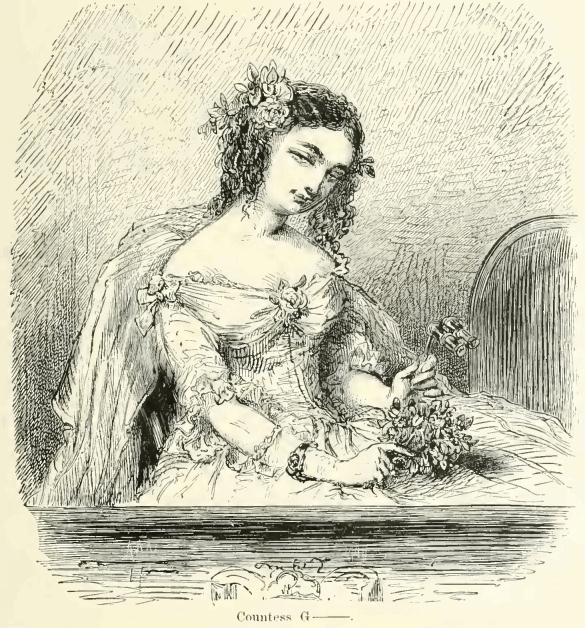
\includegraphics[width=\textwidth]{20143m.jpg}
\end{figure}

“And you will probably find your theme ill-chosen.”

“But,” said Albert, breaking in upon his discourse, “never mind the
past; let us only remember the present. Are you not going to keep your
promise of introducing me to the fair subject of our remarks?”

“Certainly, directly the curtain falls on the stage.”

“What a confounded long time this first act lasts. I believe, on my
soul, that they never mean to finish it.”

“Oh, yes, they will; only listen to that charming finale. How
exquisitely Coselli sings his part.”

“But what an awkward, inelegant fellow he is.”

“Well, then, what do you say to La Specchia? Did you ever see anything
more perfect than her acting?”

“Why, you know, my dear fellow, when one has been accustomed to
Malibran and Sontag, such singers as these don’t make the same
impression on you they perhaps do on others.”

“At least, you must admire Moriani’s style and execution.”

“I never fancied men of his dark, ponderous appearance singing with a
voice like a woman’s.”

“My good friend,” said Franz, turning to him, while Albert continued to
point his glass at every box in the theatre, “you seem determined not
to approve; you are really too difficult to please.”

The curtain at length fell on the performances, to the infinite
satisfaction of the Viscount of Morcerf, who seized his hat, rapidly
passed his fingers through his hair, arranged his cravat and
wristbands, and signified to Franz that he was waiting for him to lead
the way.

Franz, who had mutely interrogated the countess, and received from her
a gracious smile in token that he would be welcome, sought not to
retard the gratification of Albert’s eager impatience, but began at
once the tour of the house, closely followed by Albert, who availed
himself of the few minutes required to reach the opposite side of the
theatre to settle the height and smoothness of his collar, and to
arrange the lappets of his coat. This important task was just completed
as they arrived at the countess’s box.

At the knock, the door was immediately opened, and the young man who
was seated beside the countess, in obedience to the Italian custom,
instantly rose and surrendered his place to the strangers, who, in
turn, would be expected to retire upon the arrival of other visitors.

Franz presented Albert as one of the most distinguished young men of
the day, both as regarded his position in society and extraordinary
talents; nor did he say more than the truth, for in Paris and the
circle in which the viscount moved, he was looked upon and cited as a
model of perfection. Franz added that his companion, deeply grieved at
having been prevented the honor of being presented to the countess
during her sojourn in Paris, was most anxious to make up for it, and
had requested him (Franz) to remedy the past misfortune by conducting
him to her box, and concluded by asking pardon for his presumption in
having taken it upon himself to do so.

The countess, in reply, bowed gracefully to Albert, and extended her
hand with cordial kindness to Franz; then, inviting Albert to take the
vacant seat beside her, she recommended Franz to take the next best, if
he wished to view the ballet, and pointed to the one behind her own
chair.

Albert was soon deeply engrossed in discoursing upon Paris and Parisian
matters, speaking to the countess of the various persons they both knew
there. Franz perceived how completely he was in his element; and,
unwilling to interfere with the pleasure he so evidently felt, took up
Albert’s glass, and began in his turn to survey the audience.

Sitting alone, in the front of a box immediately opposite, but situated
on the third row, was a woman of exquisite beauty, dressed in a Greek
costume, which evidently, from the ease and grace with which she wore
it, was her national attire. Behind her, but in deep shadow, was the
outline of a masculine figure; but the features of this latter
personage it was not possible to distinguish. Franz could not forbear
breaking in upon the apparently interesting conversation passing
between the countess and Albert, to inquire of the former if she knew
who was the fair Albanian opposite, since beauty such as hers was well
worthy of being observed by either sex.

“All I can tell about her,” replied the countess, “is, that she has
been at Rome since the beginning of the season; for I saw her where she
now sits the very first night of the season, and since then she has
never missed a performance. Sometimes she is accompanied by the person
who is now with her, and at others she is merely attended by a black
servant.”

“And what do you think of her personal appearance?”

“Oh, I consider her perfectly lovely—she is just my idea of what Medora
must have been.”

Franz and the countess exchanged a smile, and then the latter resumed
her conversation with Albert, while Franz returned to his previous
survey of the house and company. The curtain rose on the ballet, which
was one of those excellent specimens of the Italian school, admirably
arranged and put on the stage by Henri, who has established for himself
a great reputation throughout Italy for his taste and skill in the
choreographic art—one of those masterly productions of grace, method,
and elegance in which the whole \textit{corps de ballet}, from the principal
dancers to the humblest supernumerary, are all engaged on the stage at
the same time; and a hundred and fifty persons may be seen exhibiting
the same attitude, or elevating the same arm or leg with a simultaneous
movement, that would lead you to suppose that but one mind, one act of
volition, influenced the moving mass.

The ballet was called \textit{Poliska}.

However much the ballet might have claimed his attention, Franz was too
deeply occupied with the beautiful Greek to take any note of it; while
she seemed to experience an almost childlike delight in watching it,
her eager, animated looks contrasting strongly with the utter
indifference of her companion, who, during the whole time the piece
lasted, never even moved, not even when the furious, crashing din
produced by the trumpets, cymbals, and Chinese bells sounded their
loudest from the orchestra. Of this he took no heed, but was, as far as
appearances might be trusted, enjoying soft repose and bright celestial
dreams.

The ballet at length came to a close, and the curtain fell amid the
loud, unanimous plaudits of an enthusiastic and delighted audience.

Owing to the very judicious plan of dividing the two acts of the opera
with a ballet, the pauses between the performances are very short, the
singers in the opera having time to repose themselves and change their
costume, when necessary, while the dancers are executing their
pirouettes and exhibiting their graceful steps.

The overture to the second act began; and, at the first sound of the
leader’s bow across his violin, Franz observed the sleeper slowly arise
and approach the Greek girl, who turned around to say a few words to
him, and then, leaning forward again on the railing of her box, she
became as absorbed as before in what was going on.

The countenance of the person who had addressed her remained so
completely in the shade, that, though Franz tried his utmost, he could
not distinguish a single feature. The curtain rose, and the attention
of Franz was attracted by the actors; and his eyes turned from the box
containing the Greek girl and her strange companion to watch the
business of the stage.

Most of my readers are aware that the second act of \textit{Parisina} opens
with the celebrated and effective duet in which Parisina, while
sleeping, betrays to Azzo the secret of her love for Ugo. The injured
husband goes through all the emotions of jealousy, until conviction
seizes on his mind, and then, in a frenzy of rage and indignation, he
awakens his guilty wife to tell her that he knows her guilt and to
threaten her with his vengeance.

This duet is one of the most beautiful, expressive and terrible
conceptions that has ever emanated from the fruitful pen of Donizetti.
Franz now listened to it for the third time; yet its notes, so tenderly
expressive and fearfully grand as the wretched husband and wife give
vent to their different griefs and passions, thrilled through the soul
of Franz with an effect equal to his first emotions upon hearing it.
Excited beyond his usual calm demeanor, Franz rose with the audience,
and was about to join the loud, enthusiastic applause that followed;
but suddenly his purpose was arrested, his hands fell by his sides, and
the half-uttered “bravos” expired on his lips.

The occupant of the box in which the Greek girl sat appeared to share
the universal admiration that prevailed; for he left his seat to stand
up in front, so that, his countenance being fully revealed, Franz had
no difficulty in recognizing him as the mysterious inhabitant of Monte
Cristo, and the very same person he had encountered the preceding
evening in the ruins of the Colosseum, and whose voice and figure had
seemed so familiar to him.

All doubt of his identity was now at an end; his singular host
evidently resided at Rome. The surprise and agitation occasioned by
this full confirmation of Franz’s former suspicion had no doubt
imparted a corresponding expression to his features; for the countess,
after gazing with a puzzled look at his face, burst into a fit of
laughter, and begged to know what had happened.

“Countess,” returned Franz, totally unheeding her raillery, “I asked
you a short time since if you knew any particulars respecting the
Albanian lady opposite; I must now beseech you to inform me who and
what is her husband?”

“Nay,” answered the countess, “I know no more of him than yourself.”

“Perhaps you never before noticed him?”

“What a question—so truly French! Do you not know that we Italians have
eyes only for the man we love?”

“True,” replied Franz.

“All I can say is,” continued the countess, taking up the \textit{lorgnette},
and directing it toward the box in question, “that the gentleman, whose
history I am unable to furnish, seems to me as though he had just been
dug up; he looks more like a corpse permitted by some friendly
grave-digger to quit his tomb for a while, and revisit this earth of
ours, than anything human. How ghastly pale he is!”

“Oh, he is always as colorless as you now see him,” said Franz.

“Then you know him?” almost screamed the countess. “Oh, pray do, for
heaven’s sake, tell us all about—is he a vampire, or a resuscitated
corpse, or what?”

“I fancy I have seen him before; and I even think he recognizes me.”

“And I can well understand,” said the countess, shrugging up her
beautiful shoulders, as though an involuntary shudder passed through
her veins, “that those who have once seen that man will never be likely
to forget him.”

The sensation experienced by Franz was evidently not peculiar to
himself; another, and wholly uninterested person, felt the same
unaccountable awe and misgiving.

“Well.” inquired Franz, after the countess had a second time directed
her \textit{lorgnette} at the box, “what do you think of our opposite
neighbor?”

\begin{figure}[ht]
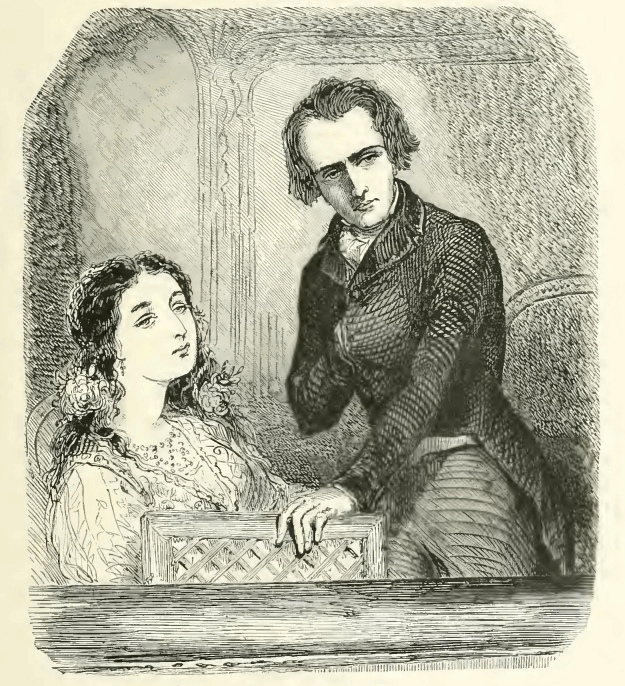
\includegraphics[width=\textwidth]{20147m.jpg}
\end{figure}

“Why, that he is no other than Lord Ruthven himself in a living form.”

This fresh allusion to Byron5 drew a smile to Franz’s countenance;
although he could but allow that if anything was likely to induce
belief in the existence of vampires, it would be the presence of such a
man as the mysterious personage before him.

“I must positively find out who and what he is,” said Franz, rising
from his seat.

“No, no,” cried the countess; “you must not leave me. I depend upon you
to escort me home. Oh, indeed, I cannot permit you to go.”

“Is it possible,” whispered Franz, “that you entertain any fear?”

“I’ll tell you,” answered the countess. “Byron had the most perfect
belief in the existence of vampires, and even assured me that he had
seen them. The description he gave me perfectly corresponds with the
features and character of the man before us. Oh, he is the exact
personification of what I have been led to expect! The coal-black hair,
large bright, glittering eyes, in which a wild, unearthly fire seems
burning,—the same ghastly paleness. Then observe, too, that the woman
with him is altogether unlike all others of her sex. She is a
foreigner—a stranger. Nobody knows who she is, or where she comes from.
No doubt she belongs to the same horrible race he does, and is, like
himself, a dealer in magical arts. I entreat of you not to go near
him—at least tonight; and if tomorrow your curiosity still continues as
great, pursue your researches if you will; but tonight you neither can
nor shall. For that purpose I mean to keep you all to myself.”

Franz protested he could not defer his pursuit till the following day,
for many reasons.

“Listen to me,” said the countess, “and do not be so very headstrong. I
am going home. I have a party at my house tonight, and therefore cannot
possibly remain till the end of the opera. Now, I cannot for one
instant believe you so devoid of gallantry as to refuse a lady your
escort when she even condescends to ask you for it.”

There was nothing else left for Franz to do but to take up his hat,
open the door of the box, and offer the countess his arm. It was quite
evident, by her manner, that her uneasiness was not feigned; and Franz
himself could not resist a feeling of superstitious dread—so much the
stronger in him, as it arose from a variety of corroborative
recollections, while the terror of the countess sprang from an
instinctive belief, originally created in her mind by the wild tales
she had listened to till she believed them truths. Franz could even
feel her arm tremble as he assisted her into the carriage. Upon
arriving at her hotel, Franz perceived that she had deceived him when
she spoke of expecting company; on the contrary, her own return before
the appointed hour seemed greatly to astonish the servants.

“Excuse my little subterfuge,” said the countess, in reply to her
companion’s half-reproachful observation on the subject; “but that
horrid man had made me feel quite uncomfortable, and I longed to be
alone, that I might compose my startled mind.”

Franz essayed to smile.

“Nay,” said she, “do not smile; it ill accords with the expression of
your countenance, and I am sure it does not spring from your heart.
However, promise me one thing.”

“What is it?”

“Promise me, I say.”

“I will do anything you desire, except relinquish my determination of
finding out who this man is. I have more reasons than you can imagine
for desiring to know who he is, from whence he came, and whither he is
going.”

“Where he comes from I am ignorant; but I can readily tell you where he
is going to, and that is down below, without the least doubt.”

“Let us only speak of the promise you wished me to make,” said Franz.

“Well, then, you must give me your word to return immediately to your
hotel, and make no attempt to follow this man tonight. There are
certain affinities between the persons we quit and those we meet
afterwards. For heaven’s sake, do not serve as a conductor between that
man and me. Pursue your chase after him tomorrow as eagerly as you
please; but never bring him near me, if you would not see me die of
terror. And now, good-night; go to your rooms, and try to sleep away
all recollections of this evening. For my own part, I am quite sure I
shall not be able to close my eyes.”

So saying, the countess quitted Franz, leaving him unable to decide
whether she were merely amusing herself at his expense, or whether her
fears and agitations were genuine.

Upon his return to the hotel, Franz found Albert in his dressing-gown
and slippers, listlessly extended on a sofa, smoking a cigar.

“My dear fellow!” cried he, springing up, “is it really you? Why, I did
not expect to see you before tomorrow.”

“My dear Albert,” replied Franz, “I am glad of this opportunity to tell
you, once and forever, that you entertain a most erroneous notion
concerning Italian women. I should have thought the continual failures
you have met with in all your own love affairs might have taught you
better by this time.”

“Upon my soul, these women would puzzle the very Devil to read them
aright. Why, here—they give you their hand—they press yours in
return—they keep up a whispering conversation—permit you to accompany
them home. Why, if a Parisian were to indulge in a quarter of these
marks of flattering attention, her reputation would be gone forever.”

“And the very reason why the women of this fine country, ‘where sounds
the \textit{si},’ as Dante writes, put so little restraint on their words and
actions, is because they live so much in public, and have really
nothing to conceal. Besides, you must have perceived that the countess
was really alarmed.”

“At what? At the sight of that respectable gentleman sitting opposite
to us in the same box with the lovely Greek girl? Now, for my part, I
met them in the lobby after the conclusion of the piece; and hang me,
if I can guess where you took your notions of the other world from. I
can assure you that this hobgoblin of yours is a deuced fine-looking
fellow—admirably dressed. Indeed, I feel quite sure, from the cut of
his clothes, they are made by a first-rate Paris tailor—probably Blin
or Humann. He was rather too pale, certainly; but then, you know,
paleness is always looked upon as a strong proof of aristocratic
descent and distinguished breeding.”

Franz smiled; for he well remembered that Albert particularly prided
himself on the entire absence of color in his own complexion.

“Well, that tends to confirm my own ideas,” said Franz, “that the
countess’s suspicions were destitute alike of sense and reason. Did he
speak in your hearing? and did you catch any of his words?”

“I did; but they were uttered in the Romaic dialect. I knew that from
the mixture of Greek words. I don’t know whether I ever told you that
when I was at college I was rather—rather strong in Greek.”

“He spoke the Romaic language, did he?”

“I think so.”

“That settles it,” murmured Franz. “’Tis he, past all doubt.”

“What do you say?”

“Nothing, nothing. But tell me, what were you thinking about when I
came in?”

“Oh, I was arranging a little surprise for you.”

“Indeed. Of what nature?”

“Why, you know it is quite impossible to procure a carriage.”

“Certainly; and I also know that we have done all that human means
afforded to endeavor to get one.”

“Now, then, in this difficulty a bright idea has flashed across my
brain.”

Franz looked at Albert as though he had not much confidence in the
suggestions of his imagination.

“I tell you what, M. Franz,” cried Albert, “you deserve to be called
out for such a misgiving and incredulous glance as that you were
pleased to bestow on me just now.”

“And I promise to give you the satisfaction of a gentleman if your
scheme turns out as ingenious as you assert.”

“Well, then, hearken to me.”

“I listen.”

“You agree, do you not, that obtaining a carriage is out of the
question?”

“I do.”

“Neither can we procure horses?”

“True; we have offered any sum, but have failed.”

“Well, now, what do you say to a cart? I dare say such a thing might be
had.”

“Very possibly.”

“And a pair of oxen?”

“As easily found as the cart.”

“Then you see, my good fellow, with a cart and a couple of oxen our
business can be managed. The cart must be tastefully ornamented; and if
you and I dress ourselves as Neapolitan reapers, we may get up a
striking tableau, after the manner of that splendid picture by Léopold
Robert. It would add greatly to the effect if the countess would join
us in the costume of a peasant from Puzzoli or Sorrento. Our group
would then be quite complete, more especially as the countess is quite
beautiful enough to represent a Madonna.”

“Well,” said Franz, “this time, M. Albert, I am bound to give you
credit for having hit upon a most capital idea.”

“And quite a national one, too,” replied Albert with gratified pride.
“A mere masque borrowed from our own festivities. Ha, ha, ye Romans!
you thought to make us, unhappy strangers, trot at the heels of your
processions, like so many lazzaroni, because no carriages or horses are
to be had in your beggarly city. But you don’t know us; when we can’t
have one thing we invent another.”

“And have you communicated your triumphant idea to anybody?”

“Only to our host. Upon my return home I sent for him, and I then
explained to him what I wished to procure. He assured me that nothing
would be easier than to furnish all I desired. One thing I was sorry
for; when I bade him have the horns of the oxen gilded, he told me
there would not be time, as it would require three days to do that; so
you see we must do without this little superfluity.”

“And where is he now?”

“Who?”

“Our host.”

“Gone out in search of our equipage, by tomorrow it might be too late.”

“Then he will be able to give us an answer tonight.”

“Oh, I expect him every minute.”

At this instant the door opened, and the head of Signor Pastrini
appeared. “\textit{Permesso}?” inquired he.

“Certainly—certainly,” cried Franz. “Come in, my host.”

“Now, then,” asked Albert eagerly, “have you found the desired cart and
oxen?”

“Better than that!” replied Signor Pastrini, with the air of a man
perfectly well satisfied with himself.

“Take care, my worthy host,” said Albert, “\textit{better} is a sure enemy to
\textit{well}.”

“Let your excellencies only leave the matter to me,” returned Signor
Pastrini in a tone indicative of unbounded self-confidence.

“But what \textit{have} you done?” asked Franz. “Speak out, there’s a worthy
fellow.”

“Your excellencies are aware,” responded the landlord, swelling with
importance, “that the Count of Monte Cristo is living on the same floor
with yourselves!”

“I should think we did know it,” exclaimed Albert, “since it is owing
to that circumstance that we are packed into these small rooms, like
two poor students in the back streets of Paris.”

“When, then, the Count of Monte Cristo, hearing of the dilemma in which
you are placed, has sent to offer you seats in his carriage and two
places at his windows in the Palazzo Rospoli.” The friends looked at
each other with unutterable surprise.

“But do you think,” asked Albert, “that we ought to accept such offers
from a perfect stranger?”

“What sort of person is this Count of Monte Cristo?” asked Franz of his
host.

“A very great nobleman, but whether Maltese or Sicilian I cannot
exactly say; but this I know, that he is noble as a Borghese and rich
as a gold mine.”

“It seems to me,” said Franz, speaking in an undertone to Albert, “that
if this person merited the high panegyrics of our landlord, he would
have conveyed his invitation through another channel, and not permitted
it to be brought to us in this unceremonious way. He would have
written—or——”

At this instant someone knocked at the door.

“Come in,” said Franz.

A servant, wearing a livery of considerable style and richness,
appeared at the threshold, and, placing two cards in the landlord’s
hands, who forthwith presented them to the two young men, he said:

“Please to deliver these, from the Count of Monte Cristo to Vicomte
Albert de Morcerf and M. Franz d’Épinay. The Count of Monte Cristo,”
continued the servant, “begs these gentlemen’s permission to wait upon
them as their neighbor, and he will be honored by an intimation of what
time they will please to receive him.”

“Faith, Franz,” whispered Albert, “there is not much to find fault with
here.”

“Tell the count,” replied Franz, “that we will do ourselves the
pleasure of calling on him.”

The servant bowed and retired.

“That is what I call an elegant mode of attack,” said Albert, “You were
quite correct in what you said, Signor Pastrini. The Count of Monte
Cristo is unquestionably a man of first-rate breeding and knowledge of
the world.”

“Then you accept his offer?” said the host.

“Of course we do,” replied Albert. “Still, I must own I am sorry to be
obliged to give up the cart and the group of reapers—it would have
produced such an effect! And were it not for the windows at the Palazzo
Rospoli, by way of recompense for the loss of our beautiful scheme, I
don’t know but what I should have held on by my original plan. What say
you, Franz?”

“Oh, I agree with you; the windows in the Palazzo Rospoli alone decided
me.”

The truth was, that the mention of two places in the Palazzo Rospoli
had recalled to Franz the conversation he had overheard the preceding
evening in the ruins of the Colosseum between the mysterious unknown
and the Transteverin, in which the stranger in the cloak had undertaken
to obtain the freedom of a condemned criminal; and if this muffled-up
individual proved (as Franz felt sure he would) the same as the person
he had just seen in the Teatro Argentina, then he should be able to
establish his identity, and also to prosecute his researches respecting
him with perfect facility and freedom.

Franz passed the night in confused dreams respecting the two meetings
he had already had with his mysterious tormentor, and in waking
speculations as to what the morrow would produce. The next day must
clear up every doubt; and unless his near neighbor and would-be friend,
the Count of Monte Cristo, possessed the ring of Gyges, and by its
power was able to render himself invisible, it was very certain he
could not escape this time.

Eight o’clock found Franz up and dressed, while Albert, who had not the
same motives for early rising, was still soundly asleep. The first act
of Franz was to summon his landlord, who presented himself with his
accustomed obsequiousness.

“Pray, Signor Pastrini,” asked Franz, “is not some execution appointed
to take place today?”

“Yes, your excellency; but if your reason for inquiry is that you may
procure a window to view it from, you are much too late.”

“Oh, no,” answered Franz, “I had no such intention; and even if I had
felt a wish to witness the spectacle, I might have done so from Monte
Pincio; could I not?”

“Ah!” exclaimed mine host, “I did not think it likely your excellency
would have chosen to mingle with such a rabble as are always collected
on that hill, which, indeed, they consider as exclusively belonging to
themselves.”

“Very possibly I may not go,” answered Franz; “but in case I feel
disposed, give me some particulars of today’s executions.”

“What particulars would your excellency like to hear?”

“Why, the number of persons condemned to suffer, their names, and
description of the death they are to die.”

“That happens just lucky, your excellency! Only a few minutes ago they
brought me the \textit{tavolettas}.”

“What are they?”

“Sort of wooden tablets hung up at the corners of streets the evening
before an execution, on which is pasted up a paper containing the names
of the condemned persons, their crimes, and mode of punishment. The
reason for so publicly announcing all this is, that all good and
faithful Catholics may offer up their prayers for the unfortunate
culprits, and, above all, beseech of Heaven to grant them a sincere
repentance.”

“And these tablets are brought to you that you may add your prayers to
those of the faithful, are they?” asked Franz somewhat incredulously.

“Oh, dear, no, your excellency! I have not time for anybody’s affairs
but my own and those of my honorable guests; but I make an agreement
with the man who pastes up the papers, and he brings them to me as he
would the playbills, that in case any person staying at my hotel should
like to witness an execution, he may obtain every requisite information
concerning the time and place etc.”

“Upon my word, that is a most delicate attention on your part, Signor
Pastrini,” cried Franz.

“Why, your excellency,” returned the landlord, chuckling and rubbing
his hands with infinite complacency, “I think I may take upon myself to
say I neglect nothing to deserve the support and patronage of the noble
visitors to this poor hotel.”

“I see that plainly enough, my most excellent host, and you may rely
upon me to proclaim so striking a proof of your attention to your
guests wherever I go. Meanwhile, oblige me by a sight of one of these
\textit{tavolettas}.”

“Nothing can be easier than to comply with your excellency’s wish,”
said the landlord, opening the door of the chamber; “I have caused one
to be placed on the landing, close by your apartment.”

Then, taking the tablet from the wall, he handed it to Franz, who read
as follows:

“‘The public is informed that on Wednesday, February 23rd, being the
first day of the Carnival, executions will take place in the Piazza del
Popolo, by order of the Tribunal of the Rota, of two persons, named
Andrea Rondolo, and Peppino, otherwise called Rocca Priori; the former
found guilty of the murder of a venerable and exemplary priest, named
Don César Torlini, canon of the church of St. John Lateran; and the
latter convicted of being an accomplice of the atrocious and sanguinary
bandit, Luigi Vampa, and his band. The first-named malefactor will be
\textit{mazzolato}, the second culprit \textit{decapitato}.

“‘The prayers of all good Christians are entreated for these
unfortunate men, that it may please God to awaken them to a sense of
their guilt, and to grant them a hearty and sincere repentance for
their crimes.’”

This was precisely what Franz had heard the evening before in the ruins
of the Colosseum. No part of the programme differed,—the names of the
condemned persons, their crimes, and mode of punishment, all agreed
with his previous information. In all probability, therefore, the
Transteverin was no other than the bandit Luigi Vampa himself, and the
man shrouded in the mantle the same he had known as “Sinbad the
Sailor,” but who, no doubt, was still pursuing his philanthropic
expedition in Rome, as he had already done at Porto-Vecchio and Tunis.

Time was getting on, however, and Franz deemed it advisable to awaken
Albert; but at the moment he prepared to proceed to his chamber, his
friend entered the room in perfect costume for the day. The anticipated
delights of the Carnival had so run in his head as to make him leave
his pillow long before his usual hour.

“Now, my excellent Signor Pastrini,” said Franz, addressing his
landlord, “since we are both ready, do you think we may proceed at once
to visit the Count of Monte Cristo?”

“Most assuredly,” replied he. “The Count of Monte Cristo is always an
early riser; and I can answer for his having been up these two hours.”

“Then you really consider we shall not be intruding if we pay our
respects to him directly?”

\begin{figure}[h]
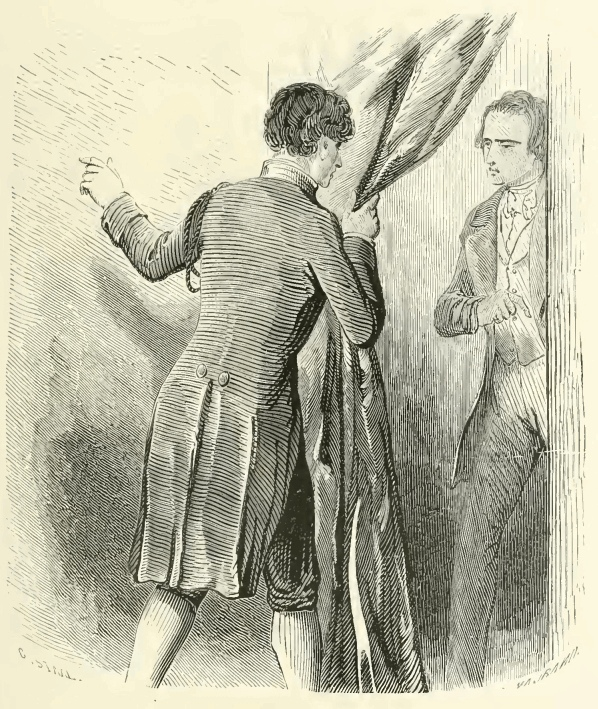
\includegraphics[width=\textwidth]{20155m.jpg}
\end{figure}

“Oh, I am quite sure. I will take all the blame on myself if you find I
have led you into an error.”

“Well, then, if it be so, are you ready, Albert?”

“Perfectly.”

“Let us go and return our best thanks for his courtesy.”

“Yes, let us do so.”

The landlord preceded the friends across the landing, which was all
that separated them from the apartments of the count, rang at the bell,
and, upon the door being opened by a servant, said:

“\textit{I signori Francesi}.”

The domestic bowed respectfully, and invited them to enter. They passed
through two rooms, furnished in a luxurious manner they had not
expected to see under the roof of Signor Pastrini, and were shown into
an elegantly fitted-up drawing-room. The richest Turkey carpets covered
the floor, and the softest and most inviting couches, easy-chairs, and
sofas, offered their high-piled and yielding cushions to such as
desired repose or refreshment. Splendid paintings by the first masters
were ranged against the walls, intermingled with magnificent trophies
of war, while heavy curtains of costly tapestry were suspended before
the different doors of the room.

“If your excellencies will please to be seated,” said the man, “I will
let the count know that you are here.”

And with these words he disappeared behind one of the tapestried
\textit{portières}. As the door opened, the sound of a \textit{guzla} reached the
ears of the young men, but was almost immediately lost, for the rapid
closing of the door merely allowed one rich swell of harmony to enter.
Franz and Albert looked inquiringly at each other, then at the gorgeous
furnishings of the apartment. Everything seemed more magnificent at a
second view than it had done at their first rapid survey.

“Well,” said Franz to his friend, “what think you of all this?”

“Why, upon my soul, my dear fellow, it strikes me that our elegant and
attentive neighbor must either be some successful stock-jobber who has
speculated in the fall of the Spanish funds, or some prince travelling
\textit{incog}.”

“Hush, hush!” replied Franz; “we shall ascertain who and what he is—he
comes!”

As Franz spoke, he heard the sound of a door turning on its hinges, and
almost immediately afterwards the tapestry was drawn aside, and the
owner of all these riches stood before the two young men. Albert
instantly rose to meet him, but Franz remained, in a manner, spellbound
on his chair; for in the person of him who had just entered he
recognized not only the mysterious visitant to the Colosseum, and the
occupant of the box at the Teatro Argentina, but also his extraordinary
host of Monte Cristo.

\begin{figure}[h]
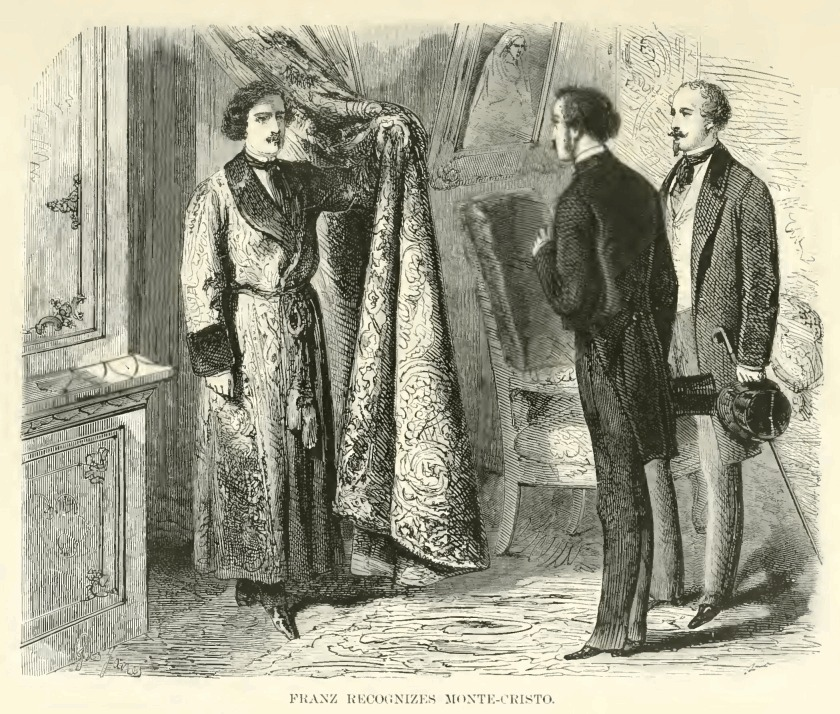
\includegraphics[width=\textwidth]{20157m.jpg}
\end{figure}
